\section{Tagger Performance} 

\frame{
    \begin{center}
        { \Huge Tagger Performance After Retuning }

        \vfill

        DISCLAIMER: All results    shown here were performed with a very limited sample size (100k events).
        The IPXD and MV2c10 algorithms were trained and tested over the same sample, rendering them extremely biased.
        Do not take these plots as measures of the absolute performance of the HLT/FTK.
        They are useful only for comparing relative performance.

    \end{center}
}
\frame{
    \frametitle{ MV2c10 Performance } 
    \begin{figure}
        \includegraphics[width=\linewidth,height=\textheight,keepaspectratio]{btag_c10_score_comparison/performance_roc_ttbar}
    \end{figure}
    \statwarn
}
\frame{
    \frametitle{ IP2D and IP3D Performance } 
    \begin{columns}
        \begin{column}{0.5\textwidth}
            \begin{figure}
                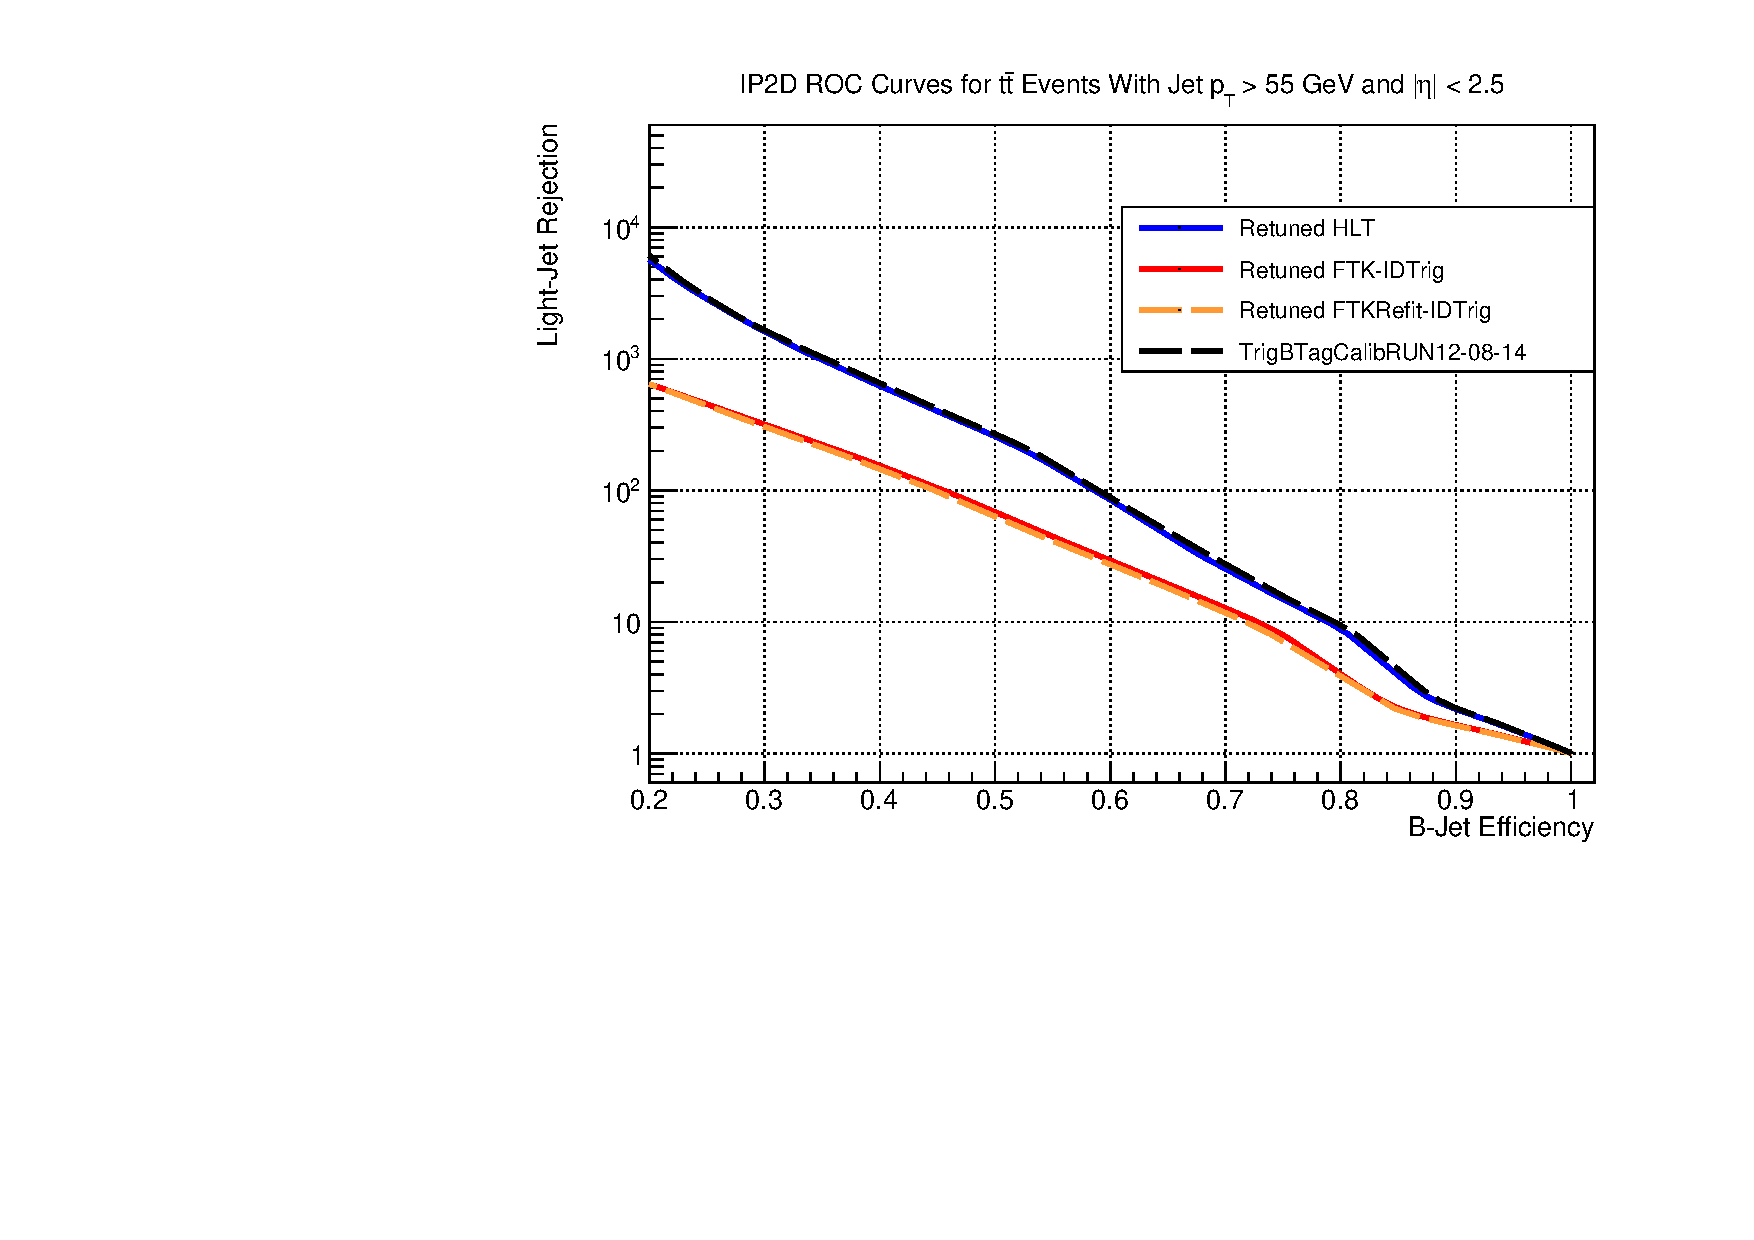
\includegraphics[width=\linewidth,height=\textheight,keepaspectratio]{ipxd_performance/performance_roc_ttbar_ip2d}
            \end{figure}
        \end{column}
        \begin{column}{0.5\textwidth}
            \begin{figure}
                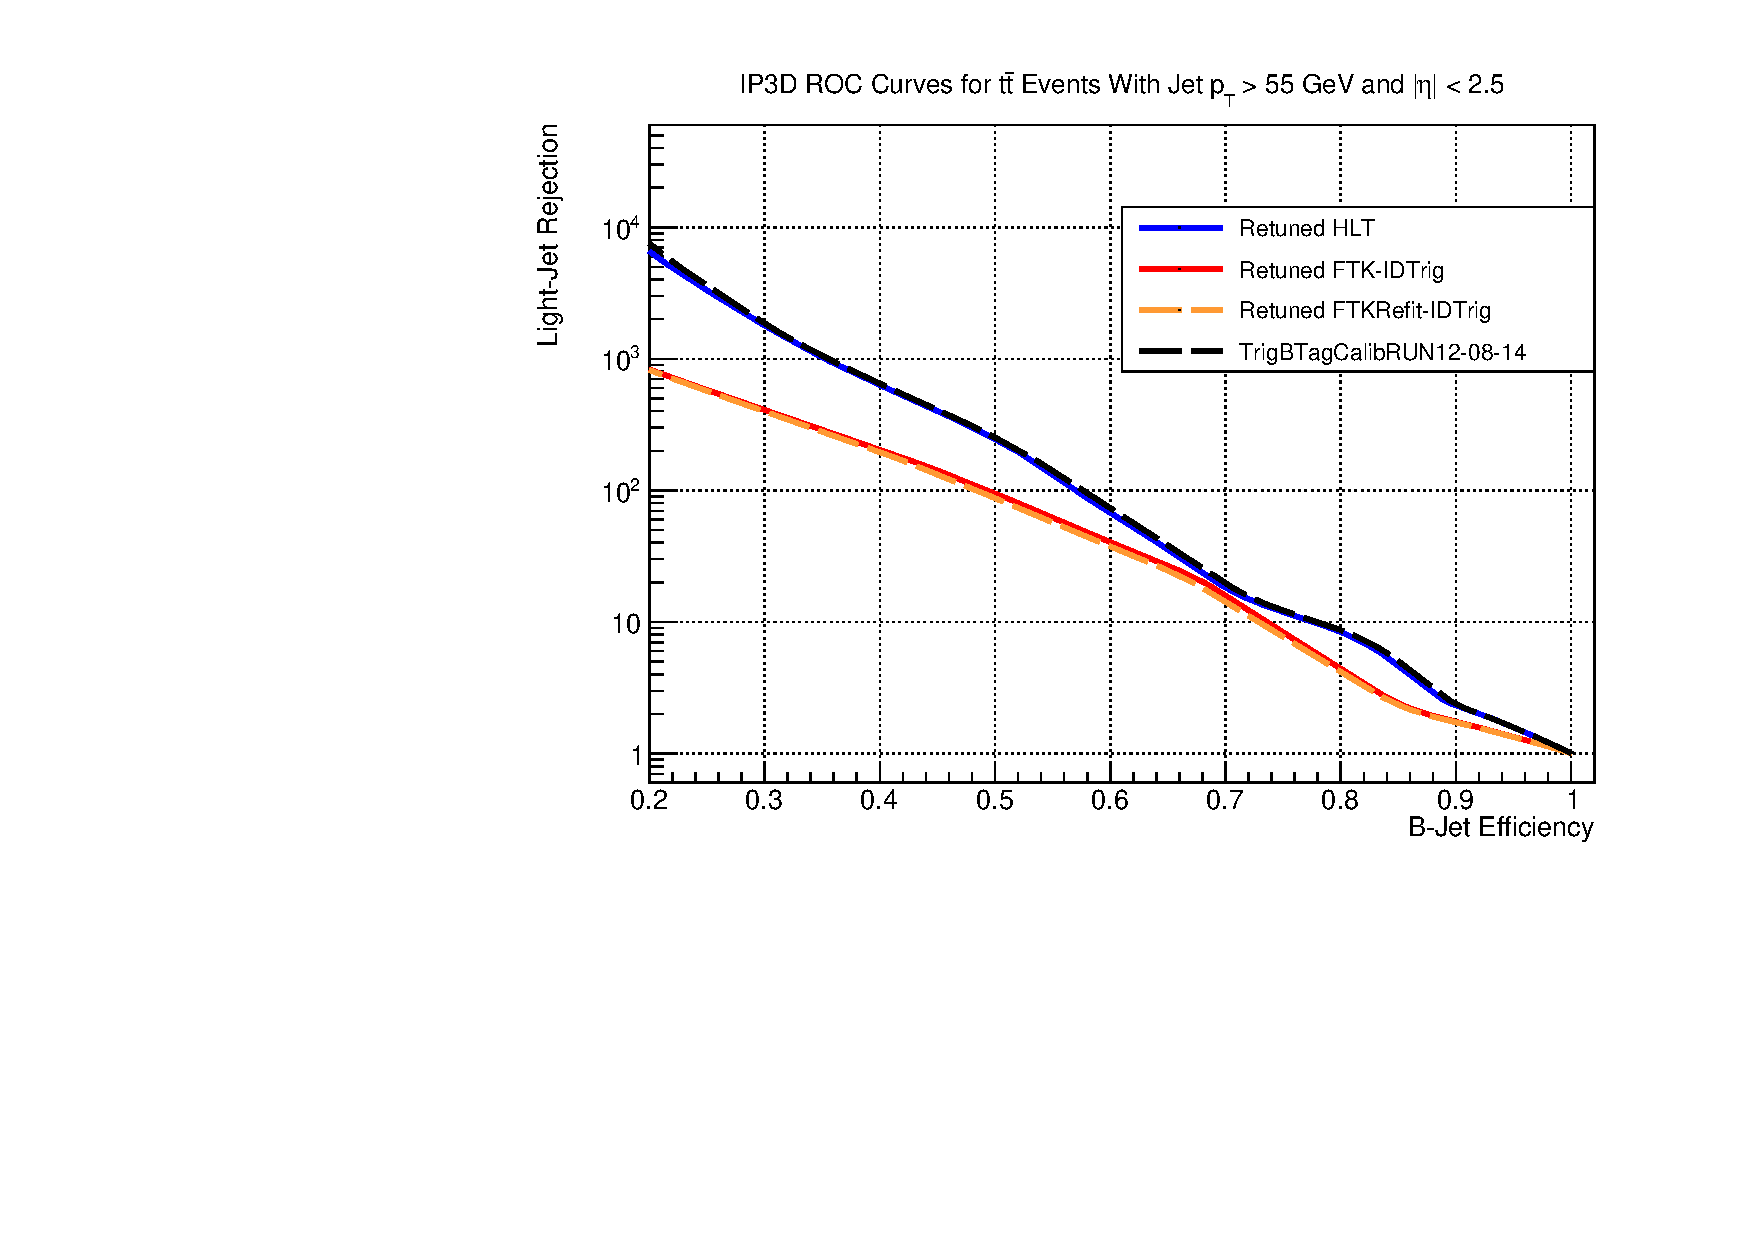
\includegraphics[width=\linewidth,height=\textheight,keepaspectratio]{ipxd_performance/performance_roc_ttbar_ip3d}
            \end{figure}
        \end{column}
    \end{columns}
    \statwarn
}


